\documentclass{article}
\usepackage[utf8]{inputenc}
\usepackage{comment}  
\usepackage{fullpage} 
\usepackage{hyperref}
\usepackage{amsmath}
\usepackage{graphicx}

\usepackage{booktabs} 

\usepackage[ruled]{algorithm2e} 
\renewcommand{\algorithmcfname}{ALGORITHM}


\begin{document}

%\maketitle
%Header-Make sure you update this information!!!!
\noindent
\large\textbf{PROBLEM 1.} \hfill \textbf{Dhruviben Modi} \\
\normalsize SOEN 6011 \hfill \textbf{40166396} \\
 SOFTWARE ENGINEERING PROCESSES \hfill Due Date: August 5, 2022 \\
\hfill Github address : git@github.com:mdhruvi/SOEN-6011-project.git

\section{Introduction}

F4: $\Gamma \left( x \right)$ which is known as Gamma function, is a generalization of the factorial function to non-integer numbers. The gamma function is defined as the improper integral of another function. It is denoted by a capital letter gamma from the Greek alphabet. \\

Let define f be the Gamma Function from A to B,therefore A is the domain and B is the  co-domain of the Gamma Function. \\
\indent(A)Domain of function: $\{x \in R^+: x > 0\}$ includes all complex numbers and the positive integer(except zero and negative integers).

(B)Co-domain of function: $(0, \infty]$\\
\indent\indent\indent When n in A is a positive integer, then the gamma function is related to the factorial function  $\Gamma(n) = (n-1)!$ \\
\indent\indent\indent When n in A for complex numbers with a positive real part, then the ${\displaystyle \Gamma (n)=\int _{0}^{\infty }x^{n-1}e^{-x}\,dx.}$

\begin{figure}[h]
    \centering
    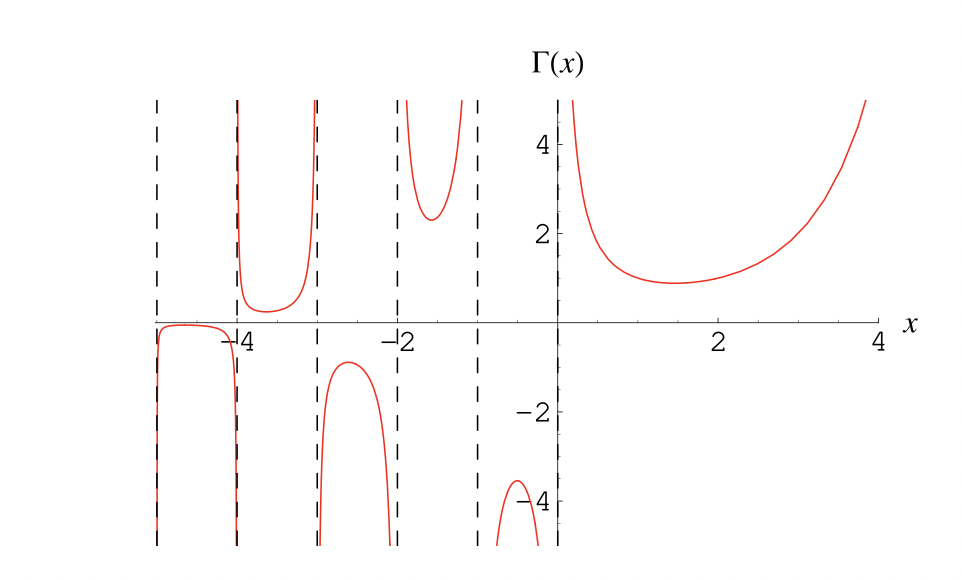
\includegraphics[width=0.4\linewidth]{Images/gammafun.png}
    \caption{Gamma Function}
    \label{fig:Gamma function}
\end{figure}

\section{Properties}
\indent\indent [1.] ${\displaystyle} n\to 0^+, {\displaystyle} \Gamma(n)\to+\infty$ \\

\indent [2.] Extreme property: a$\in\mathbf{R}$, $\lim_{n\to\infty} \frac{\Gamma(n+a)}{\Gamma(n)n^{a}} = 1, $ \\

\indent [3.] Density function: ${\displaystyle \Gamma \left(n+{\tfrac {1}{2}}\right)={\frac {(2n)!{\sqrt {\pi }}}{n!4^{n}}}}$ \\

\indent [4.] Recursive property: $\Gamma(n + 1)=n*\Gamma(n)$\\

\indent [5.] Euler's Reflection formula: $\Gamma(n)*\Gamma(1-n)=\frac{\pi}{\sin\pi n}$\\

\indent [6.] Legendre Duplication formula: $\Gamma(n)*\Gamma(n+\frac{1}{2})=2^{1-2n}*\sqrt{\pi}*\Gamma(2n)$\\

\indent [7.] For ${\lambda} > 0$, $ {\int _{0}^{\infty }x^{n-1}e^{-\lambda x}\,d} = \displaystyle \frac{\Gamma (n)}{\lambda^n}$\\

\section{Particular Values}
\indent\indent (1) $\Gamma(1) = 0! = 1$\\
\indent (2) $\Gamma(1/2) = \sqrt{\pi}$ \

\section{Context Use Model}

\begin{figure}[h]
    \centering
    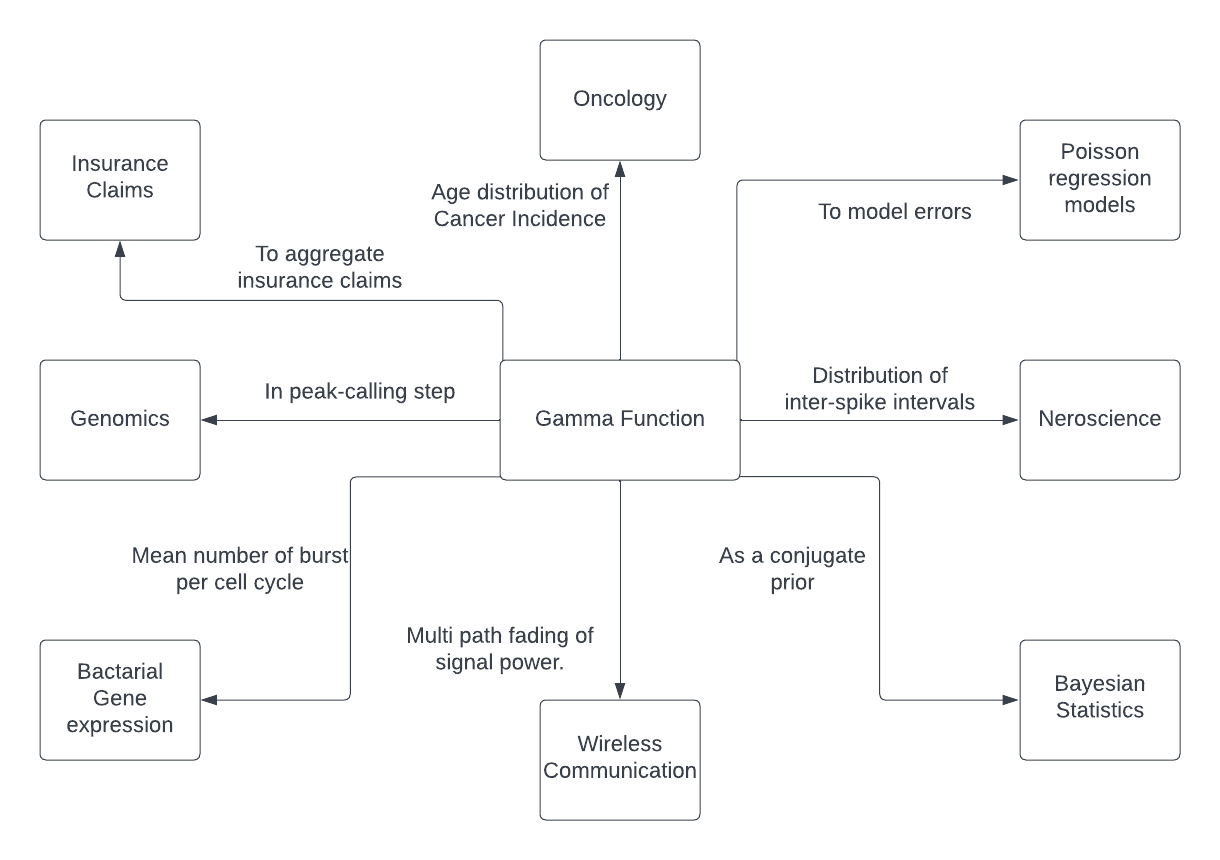
\includegraphics[width=0.9\linewidth]{Images/contextmodel.png}
    \caption{Context use model}
    \label{fig:context use model}
\end{figure}

\section{References}
\indent\indent
[En.wikipedia.org] Gamma function https://en.wikipedia.org/wiki/Gamma function\\

[Reference Resource] Function https://www.physics.uoguelph.ca/chapter-2-gamma-function\\

\end{document}
